\chapter{Montaje y funcionamiento}
\label{chap:resultado}

\lsection{Robot}
%\todo[inline]{\currentname}

Se encuentra en el lado del servidor y, funcionalmente, es una cabeza rob�tica con dos c�maras por ojos y con la capacidad de rotar sobre el eje Z (perpendicular al suelo).

\begin{figure}[H]
	\centerline{
		\mbox{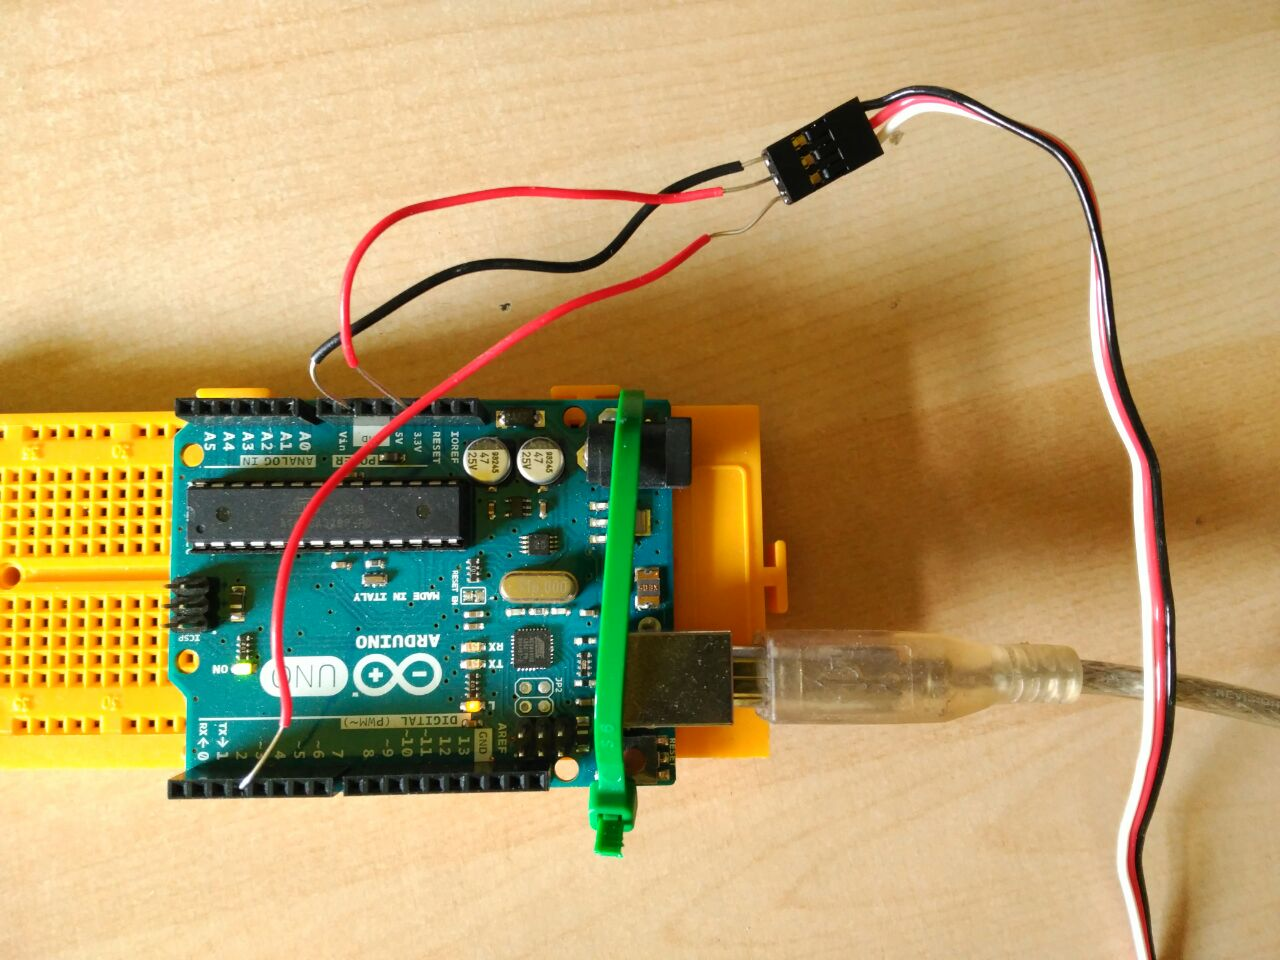
\includegraphics[width=4.00in]{images/circuito_fisico.jpg}}
	}
	\caption{\textbf{Circuito eletr�nico}: las conexiones a la placa arduino se correspondente con el dise�o en de la figura \ref{fig:circuito_arduino}. El cable conectado por la derecha de la placa se conecta al PC a trav�s de cualquier puerto USB.}
	\label{fig:circuito_fisico}
\end{figure}

\begin{figure}[p]
	\centerline{
		\mbox{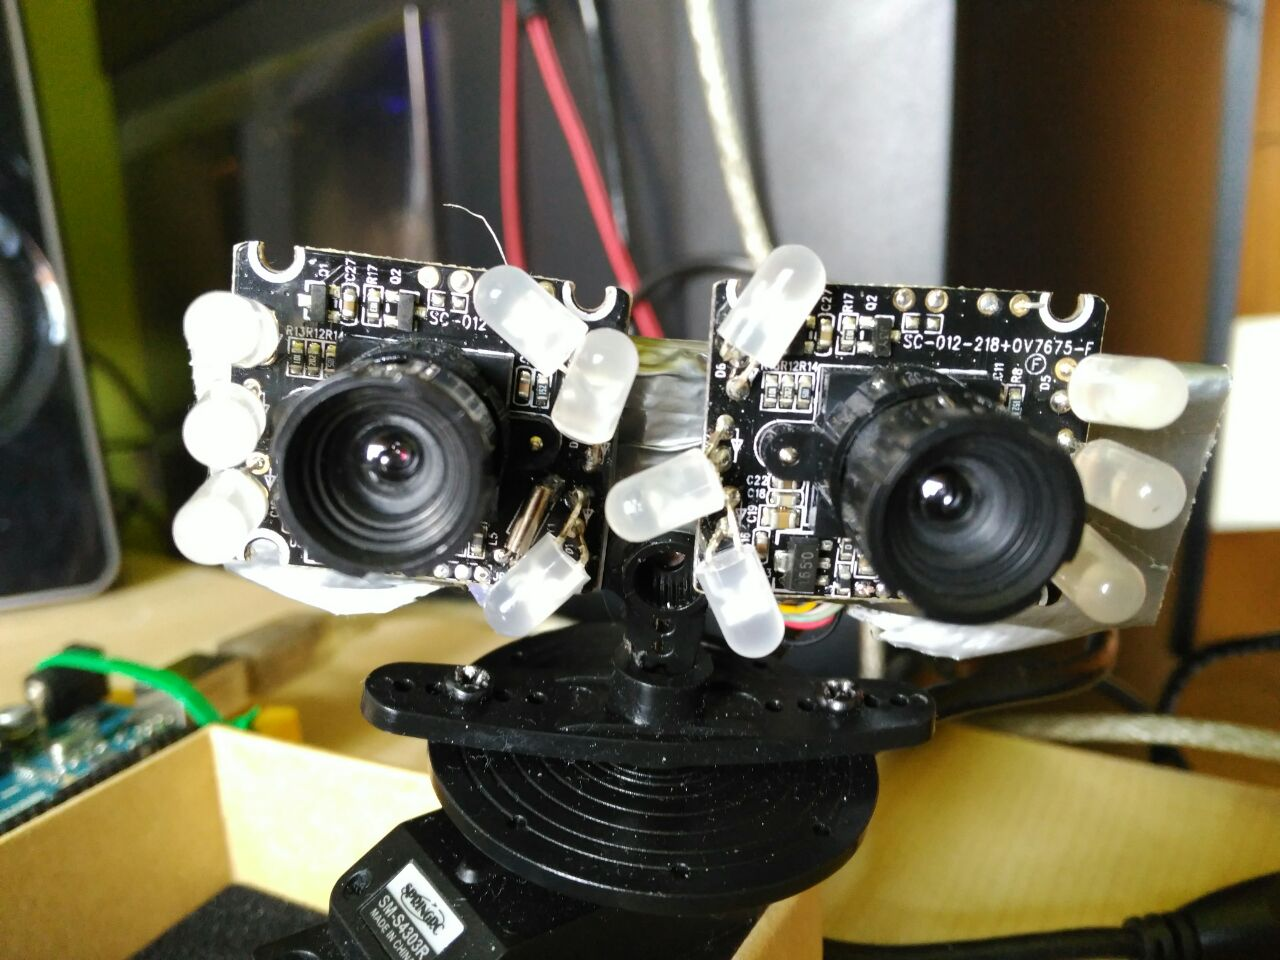
\includegraphics[width=4.00in]{images/detalle_camaras.jpg}}
	}
	\caption{\textbf{Videoc�maras}: se encuentran unidas por una estructura de cart�n fijada con cinta americana.}
	\label{fig:detalle_camaras}
\end{figure}

\begin{figure}[p]
	\centerline{
		\mbox{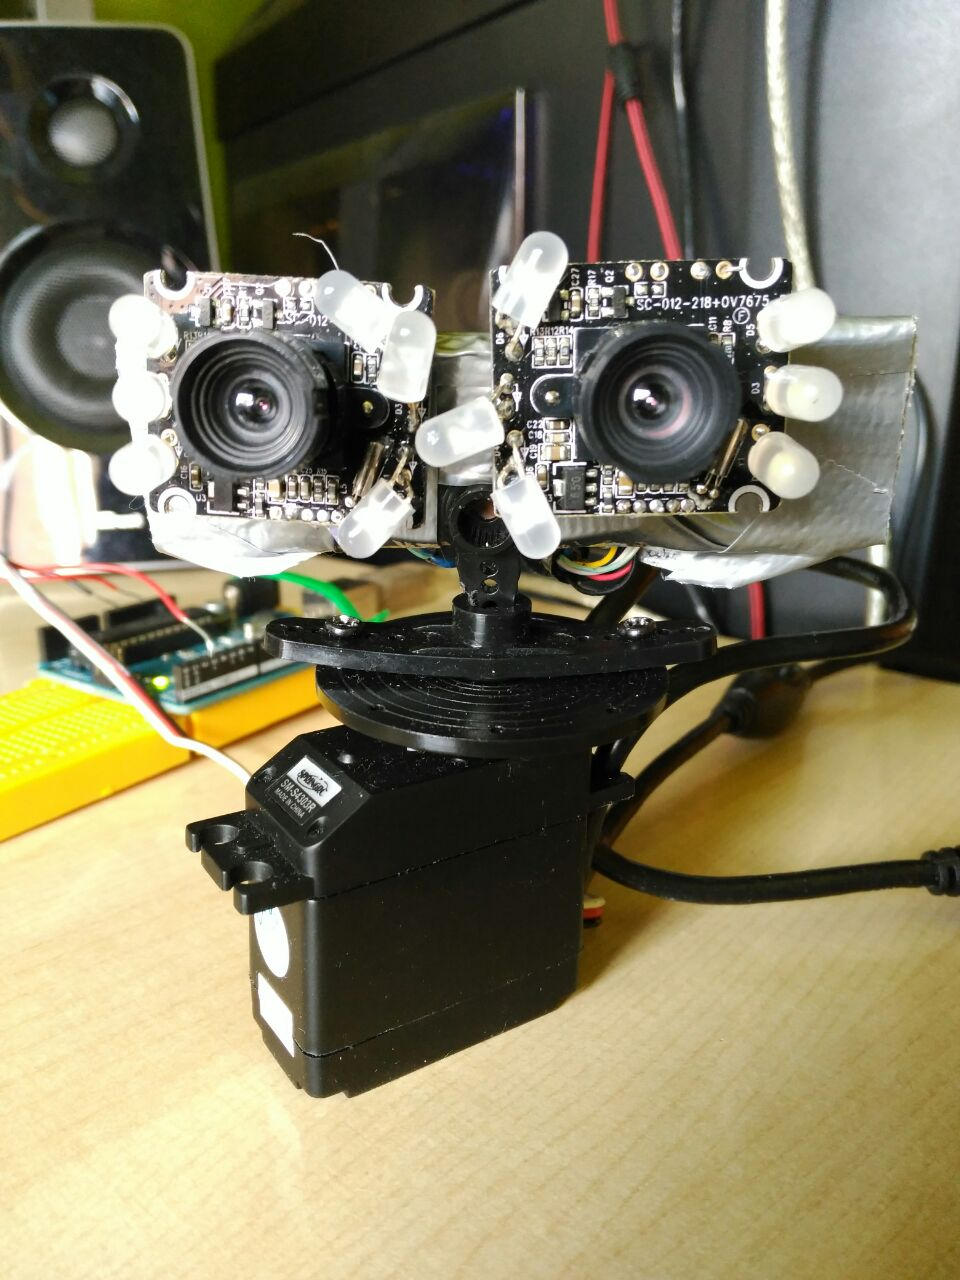
\includegraphics[width=4.00in]{images/camaras_servo.jpg}}
	}
	\caption{\textbf{Videoc�maras sobre el servomotor}: la estructura con las c�maras se coloca perpendicularmente sobre una estructura circular de un par de pulgadas de di�metro, que a su vez est� enganchada al engranaje al cual hace girar el servomotor.}
	\label{fig:camaras_servo}
\end{figure}

\newpage

\lsection{Gafas de Realidad Virtual}
%\todo[inline]{\currentname}

Las gafas de realidad virtual necesarias para este sistema no son m�s que una estructura f�sica con dos lentes y un espacio donde introducir el m�vil, de modo que el usuario pueda ver la pantalla del dispositivo a trav�s de estas lentes.



\begin{figure}[!h]
	\centering
	\centerline{
		\mbox{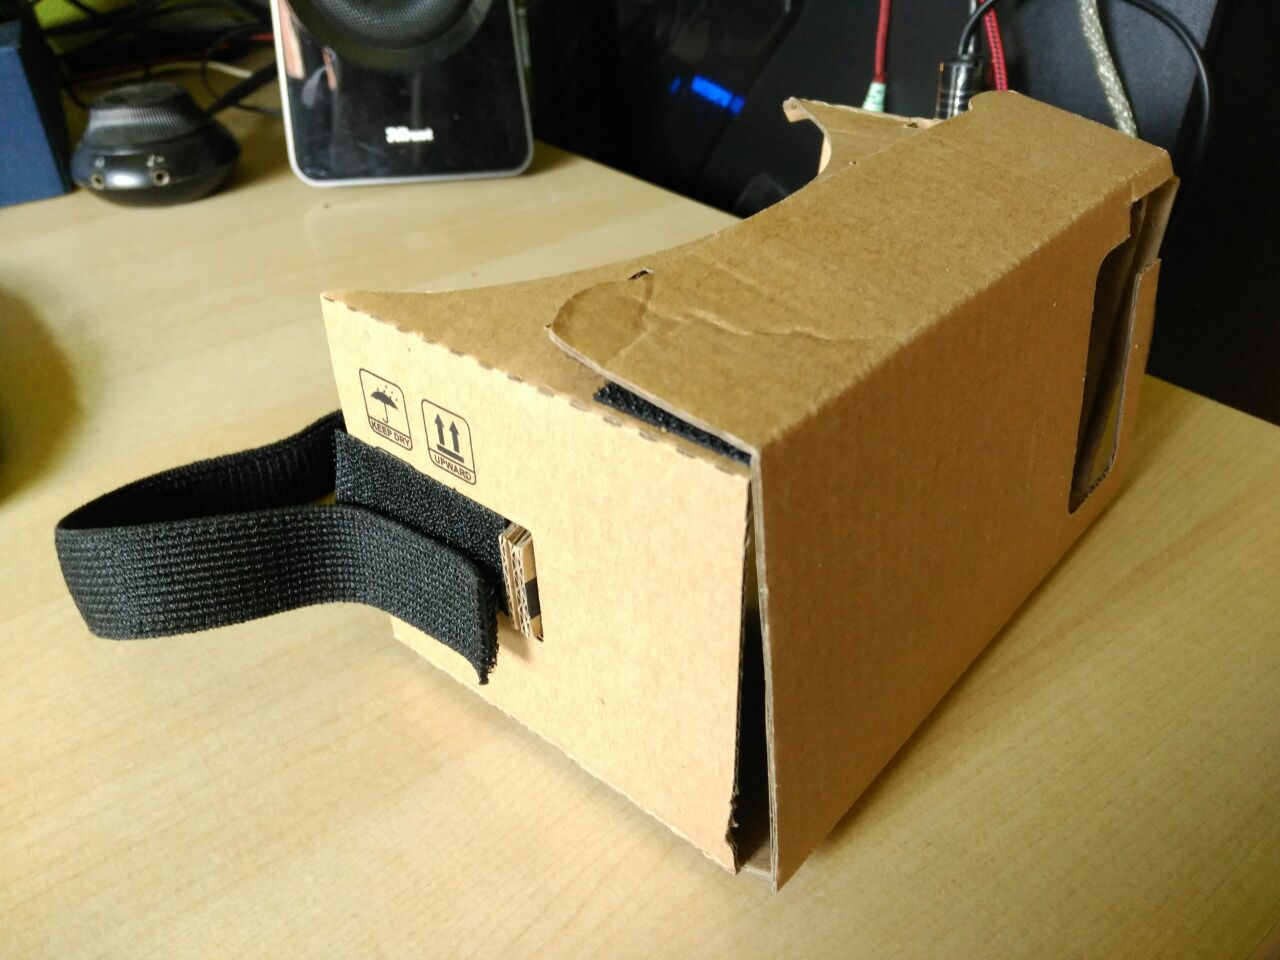
\includegraphics[width=4.00in]{images/cardboard_original.jpg}}
	}
	\caption{\textbf{Google Cardboard original}: }
	\label{fig:cardboard_original}
\end{figure}



\begin{figure}[p]
	\centerline{
		\mbox{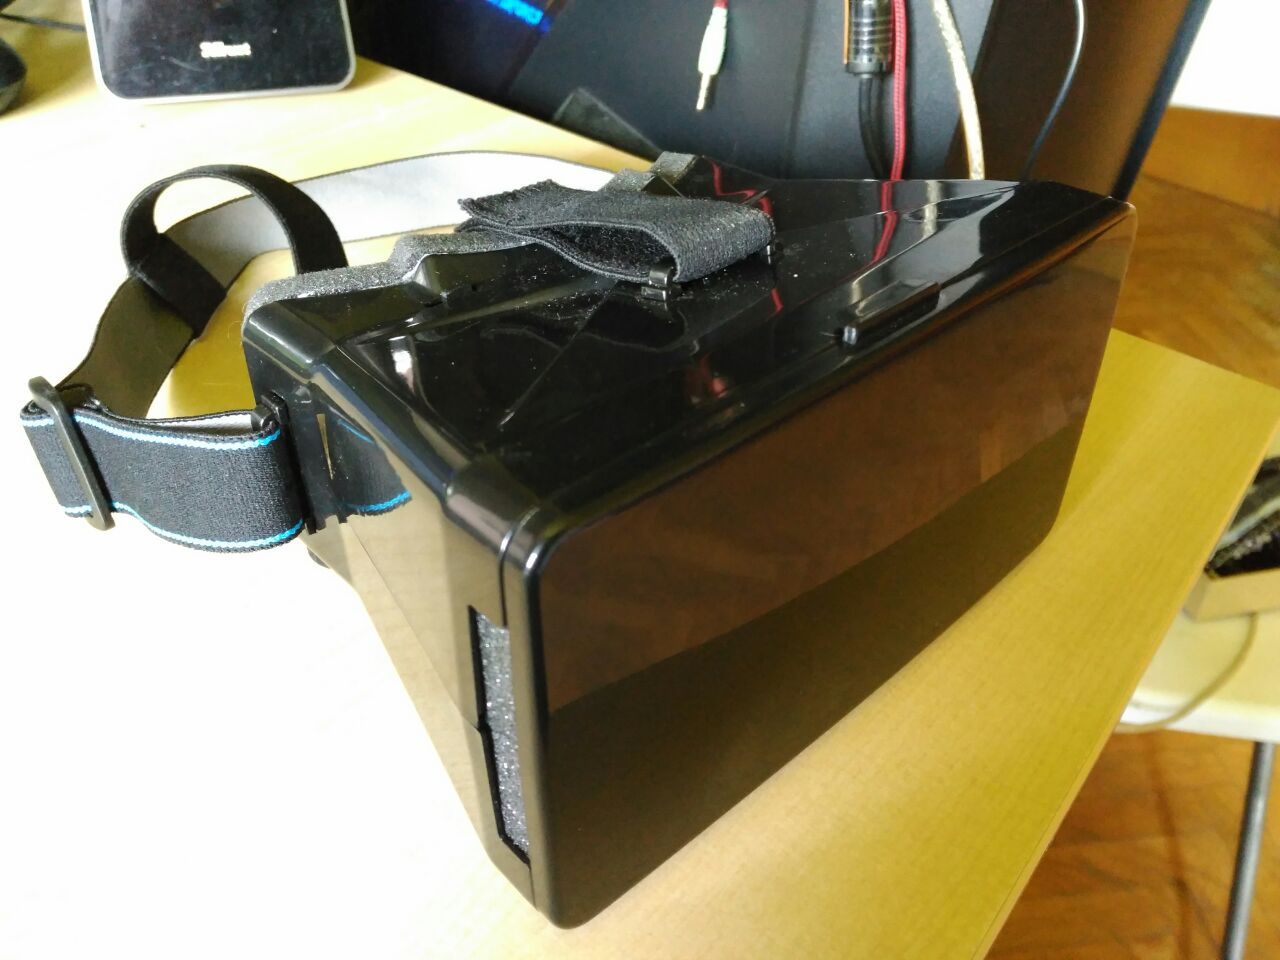
\includegraphics[width=4.00in]{images/gafas_vr_cerradas.jpg}}
	}
	\caption{\textbf{Gafas de realidad virtual de pl�stico}: estas gafas son m�s ergon�micas, ya que tiene gomaespuma en las zonas que hacen contacto con la cara y la cinta el�stica se ajusta mejor a la cabeza.}
	\label{fig:gafas_vr}
\end{figure}

\begin{figure}[p]
	\centerline{
		\mbox{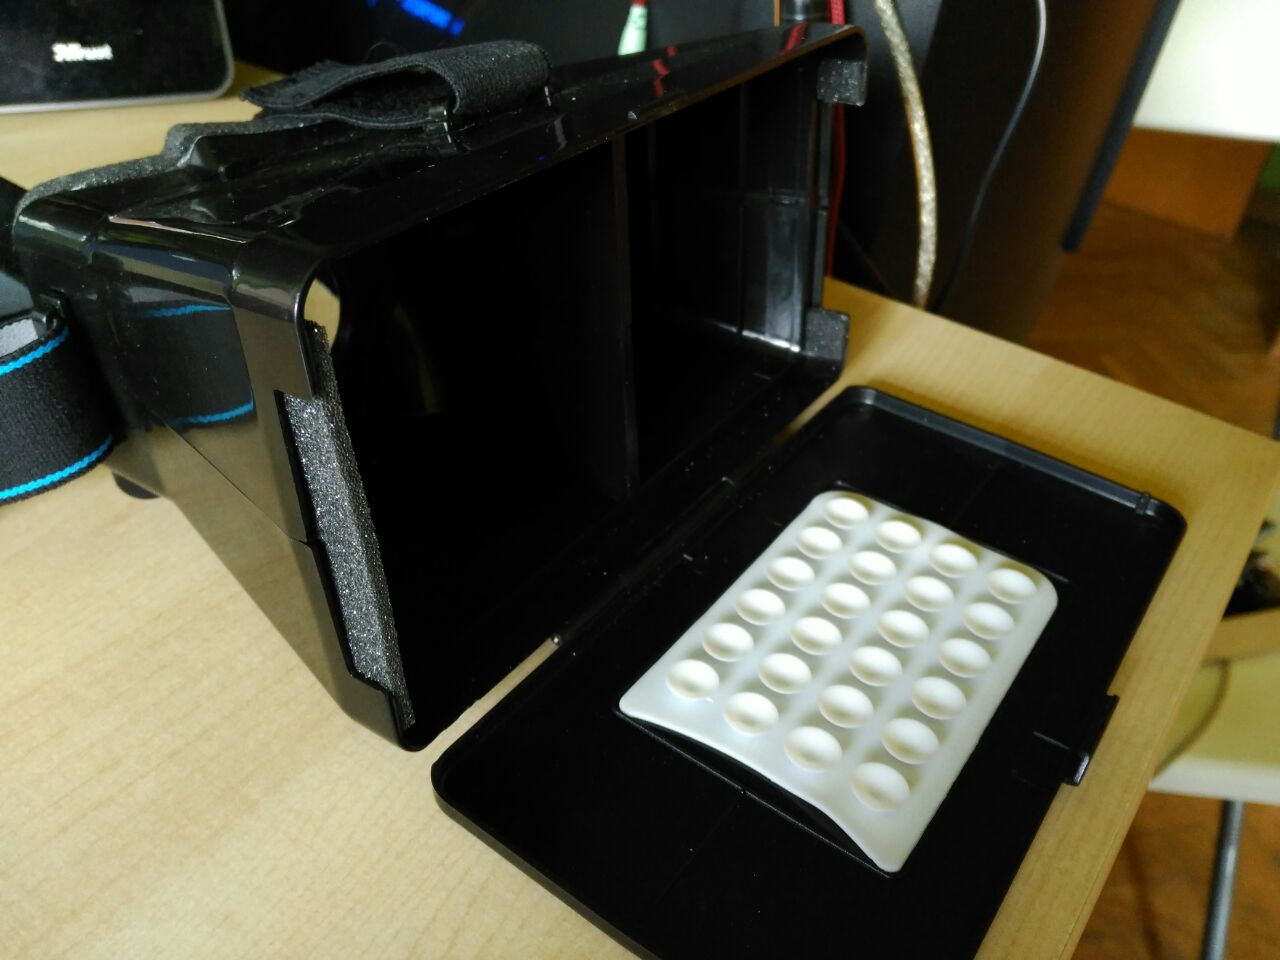
\includegraphics[width=4.00in]{images/gafas_vr_abiertas.jpg}}
	}
	\caption{\textbf{Gafas de realidad virtual de pl�stico}: la parte blanca est� compuesta de unas ventosas sobre las que se adhiere el dispositivo m�vil para que �ste no se mueva con los movimientos de la cabeza del usuario.}
	\label{fig:detalle_ventosas}
\end{figure}

\begin{figure}[p]
	\centerline{
		\mbox{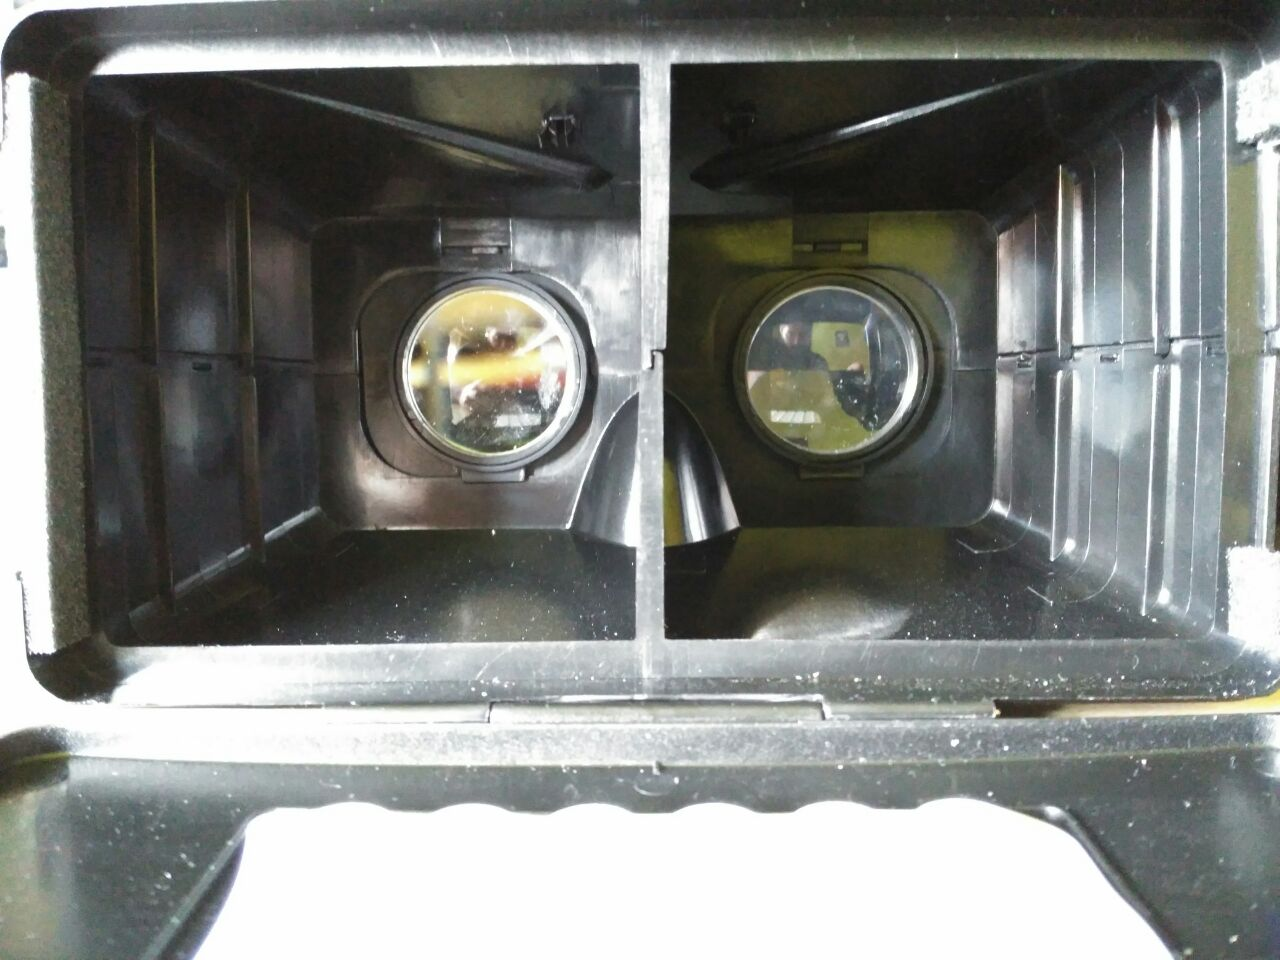
\includegraphics[width=4.00in]{images/gafas_vr_detalle_lentes.jpg}}
	}
	\caption{\textbf{Gafas de realidad virtual de pl�stico}: las lentes enfocan las im�genes que se muestran en la pantalla del dispositivo m�vil, adapt�ndolas al ojo para que el usuario pueda sentir la profundidad a partir de las dos vistas.}
	\label{fig:detalle_lentes}
\end{figure}


\begin{figure}[p]
	\centerline{
		\mbox{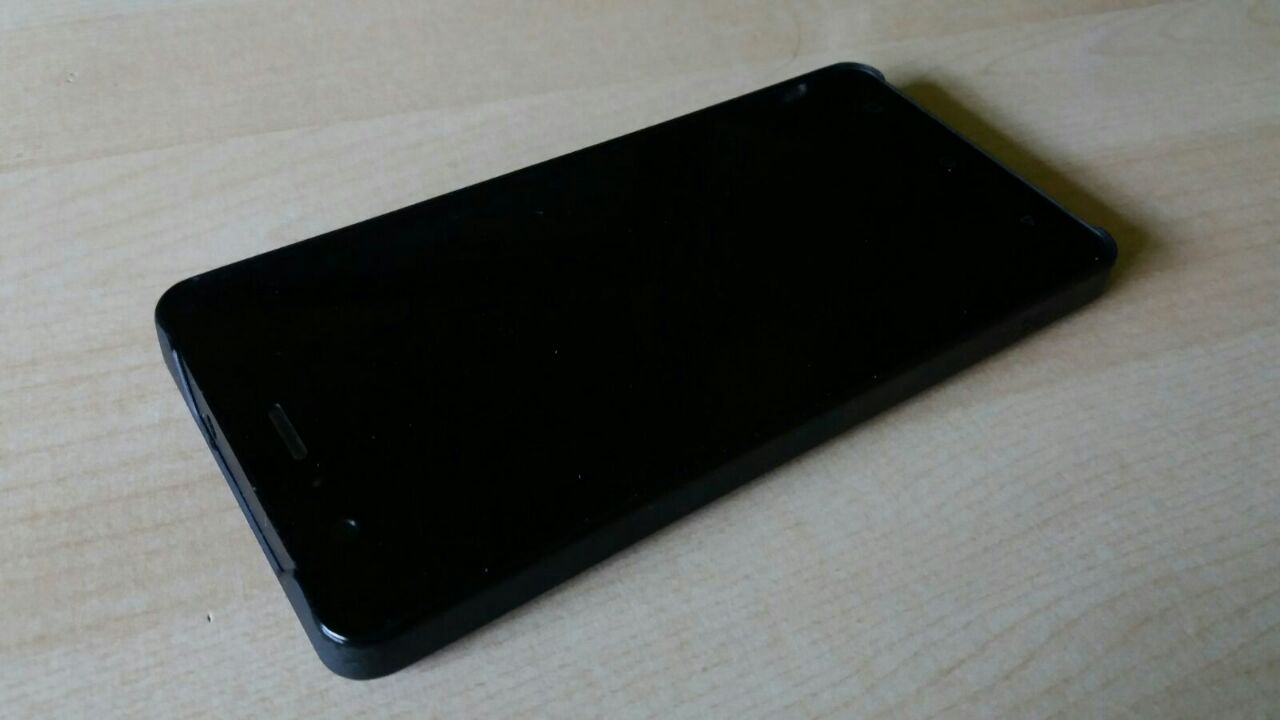
\includegraphics[width=4.00in]{images/movil.jpg}}
	}
	\caption{\textbf{\textit{Smartphone} Android}: Utiliza la versi�n Android 5.1.1 Lollipop como sistema operativo. Resoluci�n full HD (1920x1080p).}
	\label{fig:movil}
\end{figure}

\newpage

\lsection{Aplicaci�n Android}
%\todo[inline]{\currentname}
 
 A continuaci�n se muestran las capturas de pantalla correspondientes a las dos vistas de la aplicaci�n Android del cliente.


\begin{figure}[H]
	\centerline{
		\mbox{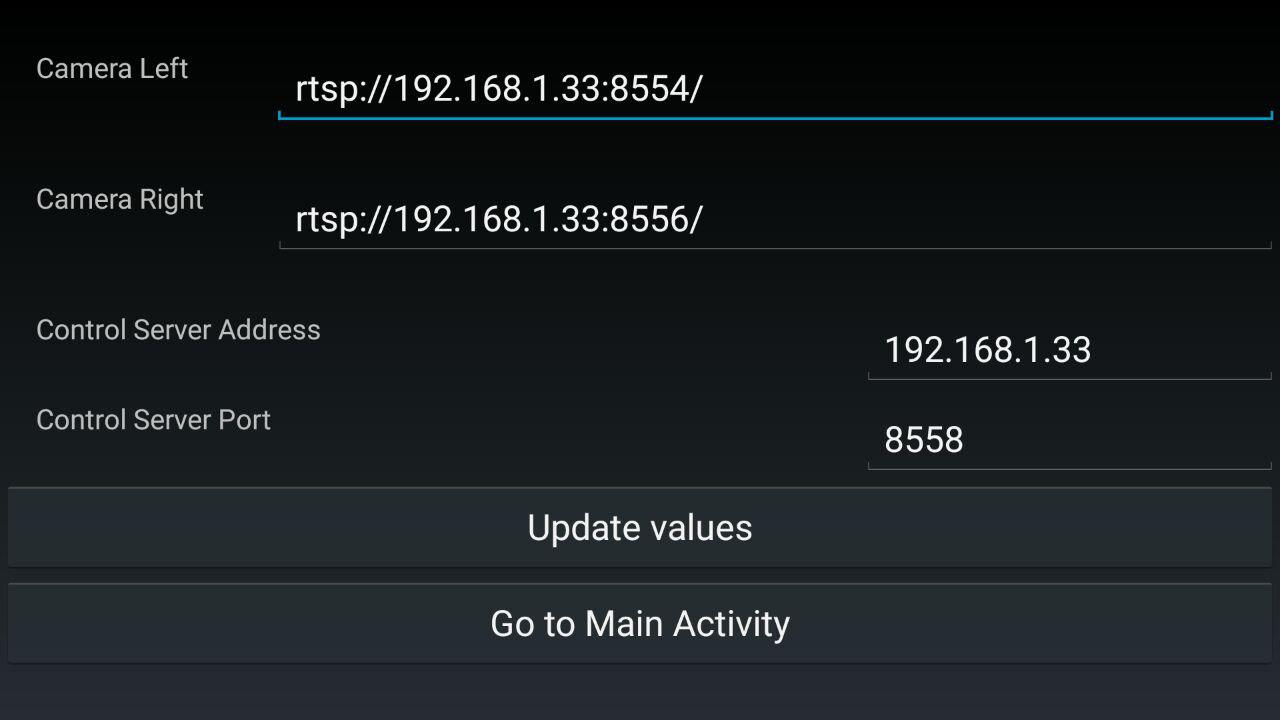
\includegraphics[width=4.00in]{images/captura_formulario.jpg}}
	}
	\caption{\textbf{Formulario de la aplicaci�n m�vil}. Permite al usuario modificar las direcciones de los tres servidores.}
	\label{fig:captura_formulario}
\end{figure}

\begin{figure}[H]
	\centerline{
		\mbox{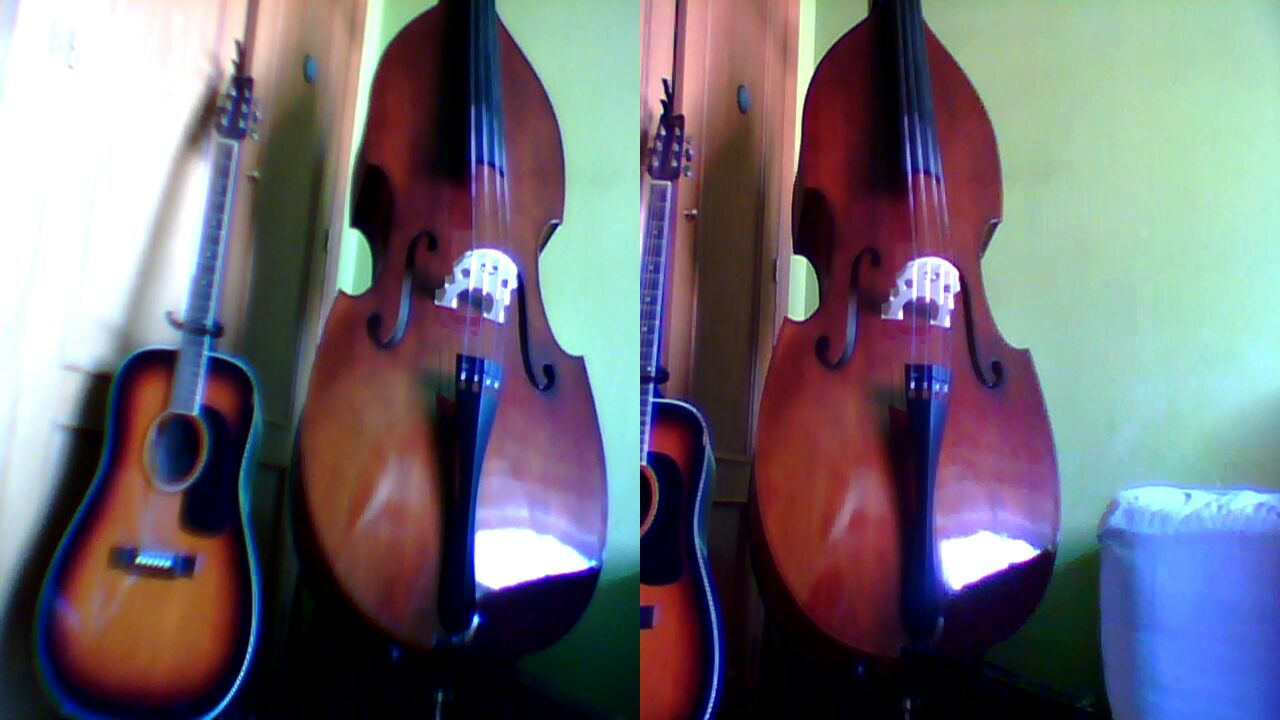
\includegraphics[width=4.00in]{images/captura_cliente_1.jpg}}
	}
	\caption{\textbf{Vista principal de la aplicaci�n m�vil}. Cada imagen se corresponde a una captura de una de las c�maras alojadas en el servidor. Esta disposici�n de las fotograf�as otorga al usuario visi�n estereosc�pica, es decir, la capacidad de sentir profundidad.}
	\label{fig:captura_cliente_1}
\end{figure}

\newpage \thispagestyle{empty} % P�gina vac�a 